This section aims at answering the research question \textbf{Q3}, while also investigating the execution time of the different stages of the visualization algorithm. In addition, results will be collected on research question \textbf{Q4}. Again, benchmark \textit{Synthetic Data B} is used. However, the validation engine is run before the experiment such that the constraint validation results are already available and linked to the samples of the dataset. 

First, a load test is conducted over the visualization algorithm running in serial and in parallel mode. In parallel mode, the plots of the nodes of the decision tree are created in parallel. The experiment is executed analog to the load test of the join experiment: On top of the number of nodes (\#nodes), constraints (\#constraints) and samples (\#samples), the maximum depth of the decision tree is varied, to see the effect of the height of the decision tree on the execution time. The visualization algorithm can be divided into different stages, whose execution times are measured individually. 

\begin{description}
\item[summarizing.] The stage summarizing the constraint validation results into frequency distribution tables. Corresponds to lines \ref{algo:tree_visualization_algorithm:summary_start} - \ref{algo:tree_visualization_algorithm:summary_end} in algorithm \ref{algo:tree_visualization_algorithm}.
\item[histogram creation.] The stage visualizing the given frequency distribution tables corresponding to the split nodes of the decision tree with histograms. Corresponds to line \ref{algo:tree_visualization_algorithm:visualize} in algorithm \ref{algo:tree_visualization_algorithm}.
\item[pie chart creation.] The stage visualizing the given frequency distribution tables corresponding to the leaves of the decision tree with pie charts. Corresponds to line \ref{algo:tree_visualization_algorithm:visualize} in algorithm \ref{algo:tree_visualization_algorithm}.
\item[writing to disk.] The stage storing the created visualizations (e.g., the pie charts and the histograms) to disk.
\item[composition.] The stage composing the stored visualizations into decision trees. Corresponds to line \ref{algo:tree_visualization_algorithm:compose} in algorithm \ref{algo:tree_visualization_algorithm}.
\item[other.] Intermediate steps (e.g., intermediate result transformations, estimation of the decision-tree-node-to-samples mapping (see section \ref{section_decision_tree_node_to_samples_mapping}))
\end{description}
The visualization algorithm makes use of the coverage concept introduced in section \ref{section_visualizing_multiple_constraint_validation_results}. The results of the experiment are depicted in Figure \ref{fig:parallelvsserial_eval} and are the basis to answer the research question \textbf{Q3}.

\begin{figure}
    \centering
    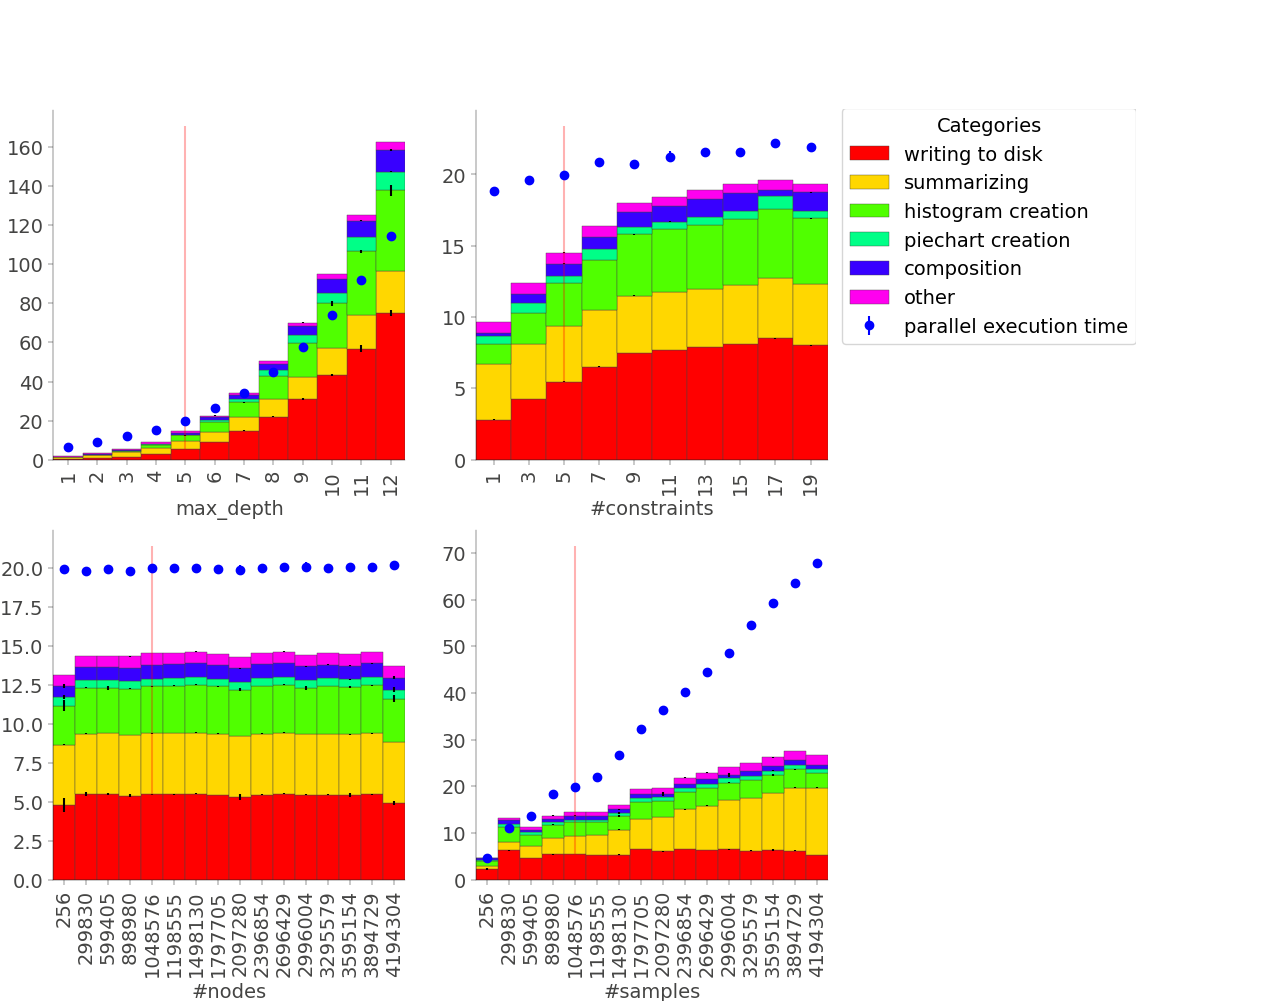
\includegraphics[width=0.8\textwidth,trim=0 0 80 70,clip]{images/evaluation/parallelVsSerialTime.png}
    \caption{Execution time [s] observed during the execution of the visualization algorithm for test beds of \textit{Synthetic Data B} with a varied number of samples, nodes, constraints and maximal depth of the trained decision tree. The bars show the execution time of the different components of the visualization algorithm running in serial mode. The dots show the overall execution time of the visualization algorithm running in parallel mode (see section \ref{section_parallel_computation}). The vertical red line marks the default value of the varied parameter as shown in table \ref{fig:parameters_used_to_generate_the_custom_dataset}.}
    \label{fig:parallelvsserial_eval}
\end{figure}

Varying the maximal depth of the decision tree, to be visualized with the annotations, corresponding to the constraint validation results, raises the execution time exponentially due to the exponentially rising number of split and leaf nodes of the decision tree. Further, the parallel node plot generation is able to improve the execution time in cases of high decision trees. For decision stumps (e.g., decision trees of depth 1) and shallow decision trees, the parallel execution time is higher than the serial execution time due to the overhead coming with multiprocessing. The overhead of the multiprocessing even raises linear with the number of samples in the dataset, although process spawning is used, which should not copy the dataset, but only the validation results summarized into frequency distribution tables to the assigned processes. In the serial execution, the execution time for summarizing the validation results increases proportional to the number of samples, while keeping the execution times of the other stages approximately constant. Therefore, the overhead added by the multiprocessing should be constant as the summarizing step is not executed in parallel; pointing to an error in the implementation of the parallel node plot generation. Varying the number of seed nodes (\#nodes) to be considered during the generation of the test bed does not impact on the execution time of the visualization algorithm. Conversely, varying the number of constraints impacts the time spend on writing to disk and creating the histograms up to a specific point, in which the complexity of the histograms stops increasing as the concept of coverage suppresses the visualization of additional less important validation results. This answers the research question \textbf{Q3}: Parallel node plot generation can impact positively in the case of high decision trees. However, with the current implementation, multiprocessing comes with a large overhead; scaling is proportional to the number of samples in the dataset. This currently limits the application since the overhead will surpass the time savings in most cases. 

As mentioned in section \ref{section_implemenation}, the visualization algorithm uses the logic provided by the dtreeviz library. However, the implementation had to be extended to support the multiprocessing and the visualization of multiple constraints. Further, the concept of frequency distribution tables as the basis of each node visualization was added for implementation convenience. It basically allowed to split the summarizing stage from the visualization stage. Finally, parts of the algorithm were improved through vectorization with NumPy (e.g., the decision-tree-node-to-sample mapping generation (see section \ref{section_decision_tree_node_to_samples_mapping})). The next experiment investigates the performance of the visualization algorithm in comparison to its original implementation in the dtreeviz library and, therefore, aims at answering the research question \textbf{Q4}.

Again, the experiment is conducted using the test beds provided by \textit{Synthetic Data B}. For comparability reasons, the visualization algorithm only has to visualize the validation results of a single constraint since the original implementation only showed the distribution of the ground truth values of the samples per node of the decision tree. In Figure \ref{fig:parallelvsserial_eval} it can be seen that the visualization of the split nodes is more costly compared to the visualization of the leaves of the decision tree. To further investigate this behavior, all test beds are used to measure the execution time of the visualization algorithm and the dtreeviz implementation; once for the visualization of the leaves only (e.g., the fancy option of the dtreeviz library turned off) and once for the entire decision tree. This time only the maximal depth of the trained decision tree and the number of samples in the dataset are varied since the number of seed nodes has shown to not impact the performance of the visualization algorithm. The results of the experiment are depicted in Figure \ref{fig:dtreevizComparison}.

\begin{figure}
    \centering
    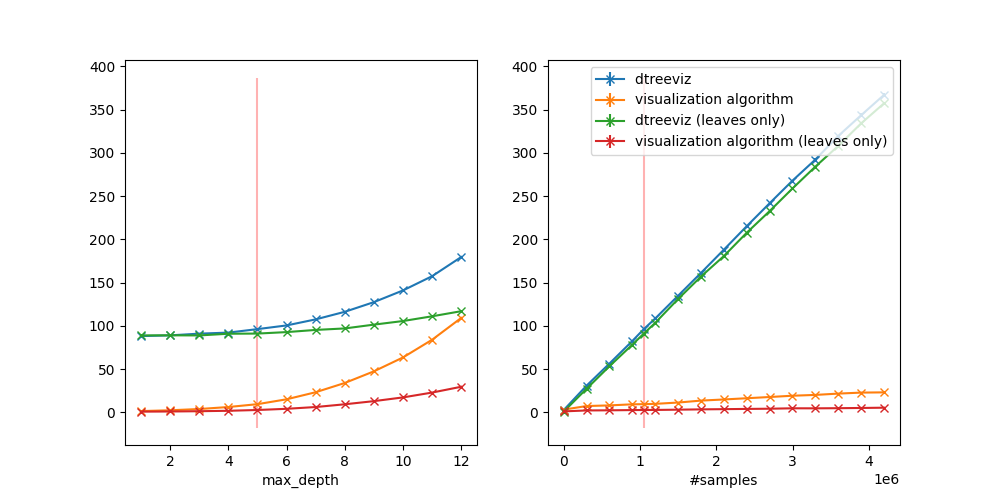
\includegraphics[width=\textwidth]{images/evaluation/dtreevizComparison.png}
    \caption{Execution time [s] observed during the execution of the visualization algorithm and it's corresponding implementation of the dtreeviz library for test beds of \textit{Synthetic Data B} with a varied number of samples in the dataset (right figure) and trained decision trees of a varied maximal depth (left figure). The vertical red line marks the default value of the varied parameter as shown in table \ref{fig:parameters_used_to_generate_the_custom_dataset}.}
    \label{fig:dtreevizComparison}
\end{figure}

At first glance, the visualization algorithm clearly outperforms the dtreeviz implementation: Varying the maximal depth or the number of samples in the dataset in all cases, the visualization algorithm is faster than the dtreeviz implementation.

For both implementations, keeping the maximal depth of the decision tree constant, the execution time scales proportionally to the number of samples. The execution time of the dtreeviz implementation and the visualization algorithm implementation increases by about $85$ and $0.9$ seconds per million samples respectively given a maximal depth of $5$ of the decision tree.

However, the visualization algorithm seems to scale slightly worse with a raising maximal depth of the decision tree. Limiting the visualization to the leaves of the decision tree reduces the execution time to the execution time needed to visualize an entire decision tree, but only of approximately half the depth. This is the expected behavior as a decision tree of height $h$ has $2^h - 1$ split nodes and $2^h$ leaf nodes. 

Nevertheless, depending on the number of samples, the visualization algorithm starts with a time advantage which can be partially derived from the improvement of the decision-tree-nodes-to-samples mapping creation. To experimentally verify this theory, a final experiment is conducted with the same setup as before, but now only measuring the execution time needed by the visualization algorithm and by the dtreeviz implementation for generating the decision-tree-node-to-samples mapping ($\Gamma_\text{nodes}$). Figure \ref{fig:load_test_join} presents the results in terms of execution time. 

\begin{figure}
    \centering
    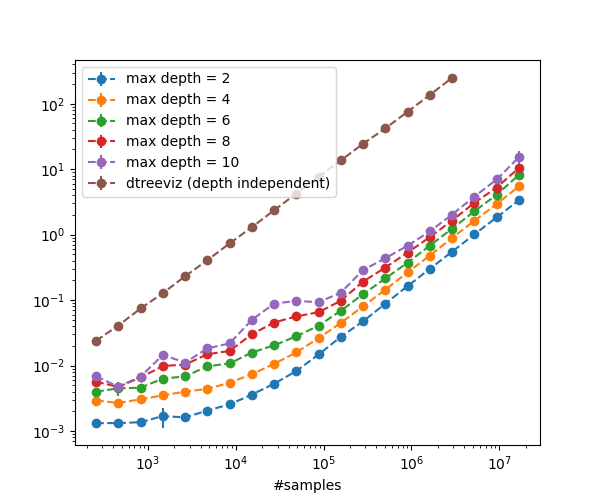
\includegraphics[width=0.6\textwidth]{images/evaluation/node_samples_exp.png}
    \caption{Execution time [s] of the generation of the decision-tree-node-to-samples mapping, observed during the execution of the visualization algorithm and its corresponding implementation of the dtreeviz library for test beds of \textit{Synthetic Data B} with a varied number of samples in the dataset and trained decision trees of a varied maximal depth.}
    \label{fig:node_samples_eval}
\end{figure}

Indeed, the experiment shows that the improved decision-tree-nodes-to-samples mapping creation, which makes use of the vectorized code execution, is faster for the observed settings. However, the conversion shown in Figure \ref{fig:rowToColumnMajor} seems to make the creation dependent on the maximum depth of the decision tree (with the original version such a dependency was not recognized). The improvement is exponential for a relatively small number of samples but turns out to be linear for a larger number of samples. In the test beds using a million samples (e.g., the ones on the left of Figure \ref{fig:dtreevizComparison}) approximately $70$ seconds of the initial time advantage are because of the worse decision-tree-nodes-to-samples mapping creation implementation.

Therefore, the research question \textbf{Q4} can now be answered: The visualization algorithm scales considerably better w.r.t. the number of samples in the dataset. This gives the visualization algorithm an initial time advantage when testing the scalability of the visualization algorithm with respect to the maximum depth of the decision tree. However, the visualization algorithm seems to scale slightly worse with a growing height of the decision tree. 